\documentclass[12pt,amstags,fleqn]{article}
%\documentclass[12pt,amstags,fleqn]{elsarticle}

\usepackage{url}

%\usepackage[mathlf,textlf,minionint]{MinionPro} \usepackage[T1]{fontenc} \usepackage{textcomp} \usepackage{amsthm}
\usepackage{amssymb}

\usepackage{amsmath}
\usepackage{amsthm}

\usepackage{xspace}

\theoremstyle{plain}
\newtheorem{theorem}{Theorem}[section]
\newtheorem{lemma}[theorem]{Lemma}
\newtheorem{proposition}[theorem]{Proposition}
\newtheorem{corollary}[theorem]{Corollary}
\newtheorem{conjecture}[theorem]{Conjecture}
\theoremstyle{definition}
\newtheorem{definition}[theorem]{Definition}
\newtheorem{construction}[theorem]{Construction}
\newtheorem{example}[theorem]{Example}
\newtheorem{remark}[theorem]{Remark}

%  \newtheorem{theorem}{Theorem}
%  \newtheorem{lemma}[theorem]{Lemma}
%  \newtheorem{conjecture}[theorem]{Conjecture}
%  \newtheorem{example}[theorem]{Example}
%  \newdefinition{definition}{Definition}
%  \newdefinition{construction}{Construction}
%  \newdefinition{remark}{Remark}
%  %\newproof{proof}{Proof}                        
%  %\newproof{pot}{Proof of Theorem \ref{thm2}}

\newcommand{\fpf}{fixed-point-free\xspace} 
\newcommand{\fp}{fixed-point\xspace} 
\newcommand{\Fp}{Fixed-point\xspace} 

\newcommand{\Rdisjoint}{\textnormal{(R1)}\xspace}
\newcommand{\RtripA}{\textnormal{(R2)}\xspace}
\newcommand{\RtripB}{\textnormal{(R3)}\xspace}

\newcommand{\darts}{\Omega}

\def\ll{{\textstyle \ast}}
\def\rr{{\scriptscriptstyle \triangle}}

\newcommand{\opa}{\ll} 
\newcommand{\opb}{\rr} 
\newcommand{\opbvar}{\times} 

%\def\eq{\operatorname{Eq}\,}
\newcommand{\eq}{\textnormal{Eq}}

\usepackage{ifpdf}

\ifpdf
    \pdfcompresslevel=9
    \usepackage[pdftex]{graphicx}
    %\usepackage{thumbpdf}
    %\usepackage[pdftex,colorlinks,bookmarks,backref]{hyperref}
    %\usepackage[pdftex,backref]{hyperref}
    %\DeclareGraphicsRule{*}{mps}{*}{}
\else
    %\usepackage{hyperref}
    %\usepackage[dvips]{graphicx}
    %\usepackage[dvips]{color}
    %\usepackage{epsfig}
    \usepackage{graphicx}
    %\DeclareGraphicsRule{*}{eps}{*}{}
\fi



\begin{document}

\title{An enumeration of equilateral triangle dissections}
\author{\Large 
Ale\v s Dr\'apal\footnote{Supported by grant MSM 0021620839}\\
Department of Mathematics \\ Charles University \\ Sokolovsk\'a 83 \\ 186 75 Praha 8 \\ Czech Republic \\
~ \\
Carlo H\"{a}m\"{a}l\"{a}inen\footnote{Supported by Eduard \v Cech center, grant LC505.}  \\
Department of Mathematics \\ Charles University \\ Sokolovsk\'a 83 \\ 186 75 Praha 8 \\ Czech Republic \\
{\texttt carlo.hamalainen@gmail.com}\\
%
}
%   \author{Ale\v s Dr\'apal\fnref{fn1}}
%   \address{Department of Mathematics, Charles University,\\
%   Sokolovsk\'a 83, 186 75 Praha 8, Czech Republic}
%   
%   \author{Carlo H\"{a}m\"{a}l\"{a}inen\corref{cor1}\fnref{fn2}}
%   \ead{carlo.hamalainen@gmail.com}
%   \address{Department of Mathematics, Charles University,\\
%   Sokolovsk\'a 83, 186 75 Praha 8, Czech Republic}
%   
%   \fntext[fn1]{Supported by grant MSM 0021620839.}
%   \fntext[fn2]{Supported by Eduard \v Cech center, grant LC505.}
%   \cortext[cor1]{Corresponding author, {\texttt carlo.hamalainen@gmail.com}}
%   
%   %\date{}


\maketitle


\begin{abstract}
We enumerate all dissections of an equilateral triangle into smaller
equilateral triangles up to size $20$, where each triangle has integer
side lengths. A {\em perfect} dissection has no two triangles of the
same side, counting up- and down-oriented triangles as different.
We computationally prove W.~T.
Tutte's conjecture that the
smallest perfect dissection has size $15$
and we find all perfect
dissections up to size $20$.
\end{abstract}

\section{Introduction}

We are concerned with the following problem: given an equilateral
triangle $\Sigma$, find all dissections of $\Sigma$ into smaller
nonoverlapping equilateral triangles. The {\em size} of a dissection is
the number of nonoverlapping equilateral triangles. An example of such a dissection
of size $10$ is shown in Figure~\ref{exDissection}. 
It is well known that in such a dissection all triangles may be
regarded as triangles with sides of integer length.
Dissections of squares have been studied earlier~\cite{MR0003040}
as well as dissections of squares into right-angled isosceles
triangles~\cite{MR1794696}. Recently, 
Laczkovich\cite{MR1092545} studied tilings of polygons by similar
triangles. The earliest study of dissections of equilateral triangles
into equilateral triangles is by Tutte~\cite{MR0027521}. The problem of
dissecting a triangle is
different to normal tiling problems where the size of the tiles is known
in advance and the tiling area may be infinite.
%%%%%%%%%%%%%%%%%%%%%%%%%%%%%%%%%%%%%%%%%%%%%%%%%%%%%%%%%%%%%%%%%%%%%
\begin{figure}[hbt]
\begin{center}
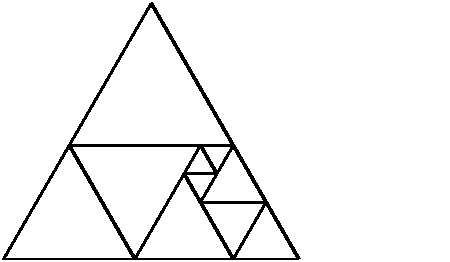
\includegraphics{dissection10_i19_r3_c1.pdf}
\end{center}
\caption{An example of an equilateral triangle dissection.}
\label{exDissection}
\end{figure}
%%%%%%%%%%%%%%%%%%%%%%%%%%%%%%%%%%%%%%%%%%%%%%%%%%%%%%%%%%%%%%%%%%%%% 
A naive approach to enumerating dissections is to first fix the sizes and
number of
the dissecting triangles. Observe that in any dissection, some triangles
will be oriented in the same way as the triangle $\Sigma$ (these are the
up-triangles) while the oppositely oriented triangles are the down-triangles.
Let $u_{s}$ and $d_{s}$ be the number of up and down triangles of side
length $s$, respectively. For any down-triangle the horizontal side is
adjacent to the horizontal side of some number of up-triangles. The
up-triangles along the bottom of $\Sigma$ are not adjacent to any
down-triangle. So if the triangle $\Sigma$ has side length $n \in
\mathbb{N}$ then
\begin{equation}\label{eqnSideSum}
\sum_{s} s u_{s} = \sum_{s} s d_{s} + n.
\end{equation}
A triangle with length ${s}$ has height $\sqrt{3}{s}/2$ and so 
the triangle areas give the relation
\begin{equation}\label{eqnAreaSum}
\sum_s u_s s^2 + \sum_s d_s s^2 = n^2.
\end{equation}
For small values of $n$ we can solve \eqref{eqnSideSum} and \eqref{eqnAreaSum}
for the permissible
size and number of up and down triangles, and this data may guide an
exhaustive search.
We will consider up and down triangles not to be congruent even
if they are of the same size. A {\em perfect tiling} or
{\em perfect dissection} has no pair of congruent triangles.
This definition of a perfect dissection arises from the fact that 
it is impossible to have a perfect dissection if orientation is
ignored~\cite{MR0003040}. This fact can also easily derived from the
results in~\cite{aleshamming}.
Tutte conjectured~\cite{MR0003040,MR0027521} that the smallest perfect
dissection has size $15$ (see also~\cite{squaring}).  Unfortunately
solving \eqref{eqnSideSum} and \eqref{eqnAreaSum} with $n = 15$ is computationally intensive and so
another approach is needed.  Using our enumerative methods we confirm Tutte's
conjecture and provide all perfect dissections up to size $20$. 


Lines parallel to the outer sides of the main triangle
that are induced by a side
of a dissecting triangle are \emph{dissecting lines}.
For any dissecting line $l$,
the union of all sides of dissecting triangles
that are incident to $l$ forms
one or more contiguous segments. If there are two or more segments,
then on $l$ there exist
two dissecting vertices such that all
triangles in between are cut by the line into two parts. If such
a situation arises for no dissecting line and if no
dissecting vertex is incident to six dissecting triangles,
then we call the dissection {\em separated}.
We enumerate all isomorphism classes of 
separated dissections up to size $24$ and provide lower 
bounds\footnote{The original version of this paper reported the counts for nonseparated dissections
as exact numbers, but this was incorrect due to the way that the code was implemented.}
on the numer of nonseparated dissections up to size $20$.

\section{Dissections and latin bitrades}

The connection between equilateral triangle dissections and latin
bitrades was first studied in~\cite{aleshamming}. The presentation here
follows~\cite{alesdissections}.  
Consider an equilateral triangle $\Sigma$ that is dissected
into a finite number of equilateral triangles. 
Dissections will be always assumed to be nontrivial so the
number of dissecting triangles is at least four. 
Denote by $a$, $b$ and $c$
the lines induced by the sides of $\Sigma$.
Each side of a dissecting triangle has to be parallel
to one of $a$, $b$, or $c$. If $X$ is a vertex
of a dissecting triangle, then $X$ is a vertex of exactly one,
three or six dissecting triangles. Suppose that there is
no vertex with six triangles and consider triples 
$(u,v,w)$ of lines that are parallel to $a$, $b$ and $c$, respectively,
and meet in  a vertex of a dissecting triangle that is not a vertex
of $\Sigma$. The set of all these triples together with the triple
$(a,b,c)$ will be denoted by $T^\ll$, and by $T^\rr$ we shall
denote the set of all triples $(u,v,w)$ of lines that are yielded 
by sides of a dissecting triangle (where $u$, $v$ and $w$ are again parallel to
$a$, $b$ and $c$, respectively). The following conditions
hold:
\begin{enumerate}
\item[(R1)] Sets $T^\ll$ and $T^\rr$ are disjoint;
\item[(R2)] for all $(p_1,p_2,p_3)\in T^\ll$ and 
all $r,s \in \{1,2,3\}$, $r \ne s$, there exists exactly one
$(q_1,q_2,q_3) \in T^\rr$ with $p_r = q_r$ and $p_s = q_s$; and
\item[(R3)] for all $(q_1,q_2,q_3)\in T^\rr$ and
all $r,s \in \{1,2,3\}$, $r \ne s$, there exists exactly one
$(p_1,p_2,p_3) \in T^\ll$ with $q_r = p_r$ and $q_s = p_s$.
\end{enumerate}

Note that (R2) would not be true if there had existed six dissecting
triangles with a common vertex. Conditions (R1--3) are, in fact, axioms
of a combinatorial object called latin bitrades
\cite[p.~148]{wanlesshandbook}. A bitrade is usually denoted
$(T^{\opa},\, T^{\opb})$. Observe that the bitrade $(T^{\opa},\,
T^{\opb})$ associated with a dissection encodes
qualitative
(structural) information about the segments and intersections of
segments in the dissection. The sizes and number of dissecting triangles
can be recovered by solving a system of equations derived from 
the bitrade (see below).

Dissections are related to a class of latin bitrades with genus~$0$. To
calculate the genus of a bitrade we use a permutation representation to
construct an oriented combinatorial surface~\cite{Dr9,hamalainen2007,ales-geometrical}.
For $r \in \{1,\, 2,\, 3\}$, define the map 
$\beta_r \colon T^{\opb} \rightarrow
T^{\opa}$ where $(a_1,\, a_2,\, a_3) \beta_r = (b_1,\, b_2,\, b_3)$ if and only if
$a_r \neq b_r$
and $a_i = b_i$ for $i \neq r$.
By (R1-3)
% Definition~\ref{defnBitradeA123}
each $\beta_r$ is a bijection.
Then
$\tau_1,\, \tau_2,\, \tau_3\colon T^{\opa} \rightarrow
T^{\opa}$ are defined by
\begin{align}
\tau_1 &= \beta_2^{-1}\beta_3, \qquad
\tau_2 = \beta_3^{-1}\beta_1, \qquad
\tau_3 = \beta_1^{-1}\beta_2. \label{eqnTau}
\end{align}
We refer to
$[\tau_1,\, \tau_2,\, \tau_3]$
as the $\tau_i$ {\em representation}. To get a combinatorial surface
from a bitrade we use the following construction:

%\begin{construction}[$\tau_i$ surface]\label{constructionTauiSurface}
\begin{construction}\label{constructionTauiSurface}
Let $[\tau_1,\, \tau_2,\, \tau_3]$ be the representation for 
a bitrade where the $\tau_i$ act on
the set $\darts$. Define
vertex, directed edge, and face sets by:
\begin{alignat*}{2}
V &= \darts \\
E &= \{ (x,y) \mid x \tau_1 = y \} \cup \{ (x,y) \mid x \tau_2 = y \} \cup \{ (x,y) \mid x \tau_3 = y \} \\
F &= \{ (x,y,z) \mid \text{ $x \tau_1 = y$, $y \tau_2 = z$, $z \tau_3 = x$} \} \\
  & \qquad \cup \{ (x_1,\, x_2,\, \dots,\, x_r) \mid \text{ $(x_1,\,
x_2,\, \dots,\, x_r)$ is a cycle of $\tau_1$ } \} \\
  & \qquad \cup \{ (x_1,\, x_2,\, \dots,\, x_r) \mid \text{ $(x_1,\,
x_2,\, \dots,\, x_r)$ is a cycle of $\tau_2$ } \} \\
  & \qquad \cup \{ (x_1,\, x_2,\, \dots,\, x_r) \mid \text{ $(x_1,\,
x_2,\, \dots,\, x_r)$ is a cycle of $\tau_3$ } \}
\end{alignat*}
where $(x_1,\, x_2,\, \dots,\, x_k)$ denotes a face with $k$~directed edges
$(x_1,\, x_2)$, $(x_2,\, x_3)$, $\dots$,
$(x_{k-1},\, x_k)$, $(x_k,\, x_1)$ for vertices
$x_1,\, \dots,\, x_k$.

The first set in the definition of $F$ is the set of {\em triangular
faces}, while the other three are the {\em $\tau_i$ faces}.
Assign triangular faces a positive (anticlockwise) orientation, and
assign
$\tau_i$ faces negative (clockwise) orientation. Now glue the faces
together where they share a common directed edge $x \tau_i = y$,
ensuring that edges come together with opposite orientation.
%(see
%Construction~\ref{constructionSAPtoMap} and 
%Example~\ref{exGluingFaces} for another example of this type of gluing process).
\end{construction}

%Theorem~\ref{theoremMapRotation} ensures that the construction does
%produce a combinatorial surface.
The orientation of a triangular face is
shown in Figure~\ref{figTwoOrientations} along with the orientation for
a $\tau_i$ face. For the sake of concreteness we have illustrated a
$6$-cycle face due to a $6$-cycle of $\tau_1$. 
Figure~\ref{figDrapalRotationScheme} shows
the rotation scheme for an arbitrary vertex in the surface.
%%%%%%%%%%%%%%%%%%%%%%%%%%%%%%%%%%%%%%%%%%%%%%%%%%%%%%%%%%%%%%%%%%%%%
\begin{figure}[htb]
\begin{center}
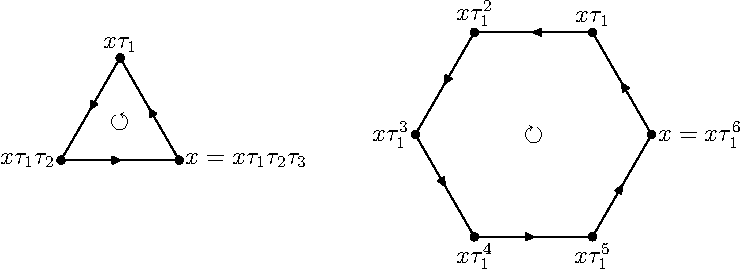
\includegraphics{drRotationScheme-1.pdf}
\end{center}
\caption{Orienting faces in the combinatorial surface.}
\label{figTwoOrientations}
\end{figure}
%%%%%%%%%%%%%%%%%%%%%%%%%%%%%%%%%%%%%%%%%%%%%%%%%%%%%%%%%%%%%%%%%%%%% 
%%%%%%%%%%%%%%%%%%%%%%%%%%%%%%%%%%%%%%%%%%%%%%%%%%%%%%%%%%%%%%%%%%%%%
\begin{figure}[htb]
\begin{center}
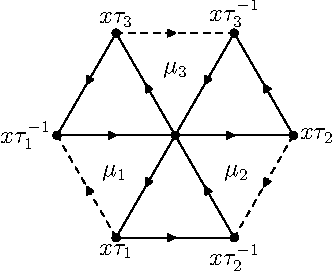
\includegraphics{drRotationScheme-2.pdf}
\end{center}
\caption{Rotation scheme for the combinatorial surface. Dashed
lines represent one or more edges, where $\mu_i$ is a cycle of $\tau_i$.
The vertex in the centre is $x$.}
\label{figDrapalRotationScheme}
\end{figure}
%%%%%%%%%%%%%%%%%%%%%%%%%%%%%%%%%%%%%%%%%%%%%%%%%%%%%%%%%%%%%%%%%%%%% 

For a bitrade $T = (T^{\opa},\, T^{\opb})$ with representation 
$[\tau_1,\, \tau_2,\, \tau_3]$
on the set $\darts$,
% = \mov(\tau_1) \cup \mov(\tau_2) \cup \mov(\tau_3)$,
define
$\text{order}(T)  = z(\tau_1) + z(\tau_2) + z(\tau_3)$, the total number
of cycles, and
$\text{size}(T) = \left| \darts \right|$, the total number of points 
that the $\tau_i$ act on. 
By some basic counting arguments we find that there are 
$\text{size}(T)$ vertices, $3 \cdot \text{size}(T)$ edges, and 
$\text{order}(T) + \text{size}(T)$ faces. Then Euler's formula
$V-E+F=2-2g$ gives
\begin{equation}\label{eqnDrapalGenus}
\text{order}(T) = \text{size}(T) + 2 - 2g
\end{equation}
where $g$ is the genus of the combinatorial surface. We say that
the bitrade $T$ has genus $g$.
A {\em spherical bitrade} has genus~$0$.

\begin{example}\label{exspherical}
The following bitrade is spherical:
\begin{align*}
T^{\opa} = 
\begin{array}{|c||c|c|c|c|c|}
\hline
\opa & 0 & 1 & 2 & 3 & 4\\
\hline
 \hline 0 & 0 & ~ & 2 & ~ & 4\\
 \hline 1 & ~ & ~ & ~ & 4 & 2\\
 \hline 2 & 1 & 3 & 0 & 2 & ~\\
 \hline 3 & 4 & 1 & ~ & 3 & ~\\
 %\hline 4 & ~ & ~ & ~ & ~ & ~ \\
\hline
\end{array}
& \quad & 
T^{\opb} = 
\begin{array}{|c||c|c|c|c|c|}
\hline
\opb & 0 & 1 & 2 & 3 & 4\\
\hline
 \hline 0 & 4 & ~ & 0 & ~ & 2\\
 \hline 1 & ~ & ~ & ~ & 2 & 4\\
 \hline 2 & 0 & 1 & 2 & 3 & ~\\
 \hline 3 & 1 & 3 & ~ & 4 & ~\\ 
%\hline 4 & ~ & ~ & ~ & ~ & ~\\
\hline
\end{array}
%\label{eqnsphericalbitrade}
\end{align*}
Here, the $\tau_i$ representation is
\begin{align*}
\tau_1 &= (000, 022, 044)(134, 142) (201,213,232,220) (304,333,311) \\
\tau_2 &= (000,304,201)(213,311)(022,220)(134,232,333)(044,142) \\
\tau_3 &= (000,220)(201,311)(022,232,142)(213,333)(044,134,304)
\end{align*}
where the triples $ijk$ refer to entries $(i,j,k) \in T^{\opa}$.
\end{example}

We will generally assume that a bitrade is {\em separated}, that is,
each row, column, and symbol is in bijection with a cycle of $\tau_1$,
$\tau_2$, and $\tau_3$, respectively.

We now describe how to go from a separated spherical latin bitrade to a
triangle dissection (for more details see~\cite{alesdissections}).  
Let $T= (T^\ll, T^\rr)$ be a latin bitrade. It is natural to have
different unknowns for rows, columns and symbols, and so we assume
that $a_i \ne b_j$ whenever $(a_1,a_2,a_3)$, $(b_1,b_2,b_3) \in T^\ll$
and $1 \le i < j \le 3$.  (If the condition is violated,  then $T$
can be replaced by an isotopic bitrade for which it is satisfied.)
Fix a triple $a = (a_1,a_2,a_3) \in T^\ll$ and form the set of equations
$\eq(T)$ consisting of
$a_1=0$, $a_2=0$, $a_3 =1$
and 
$b_1+b_2 = b_3$  if $(b_1,b_2,b_3) \neq (a_1,a_2,a_3)$
and $(b_1,b_2,b_3) \in T^\ll$.
The theorem below shows that if $T$ is a spherical latin
bitrade then $\eq(T, a)$ always has a unique solution in the rationals.
The pair $(T,a)$ will be called a \emph{pointed} bitrade.

Write
$\bar r_i$,
$\bar c_j$,
$\bar s_k$
for the solutions in $\eq(T, a)$ for row variable $r_i$, column variable
$c_j$, and symbol variable $s_k$, respectively. We say that 
a solution to $\eq(T, a)$ is {\em separated} if 
$\bar r_i \neq \bar r_{i'}$ whenever $i \neq i'$ (and similar for
columns and symbols).

For each entry $c = (c_1,c_2,c_3) \in T^\rr$ we form the triangle
$\Delta(c,a)$ which is bounded by the lines
$y = \bar c_1$,
$x = \bar c_2$,
$x + y = \bar c_3$.
%%%%%%%%%%%%%%%%%%%%%%%
Of course, it is not clear that $\Delta$ is really
a triangle, i.~e.~that the three lines do not meet in a single
point. If this happens, then we shall say that $\Delta(c,a)$ {\em degenerates}.
Let $\Delta(T,a)$ denote the subset of $T^\rr$ such that
$\Delta(c,a)$ does not degenerate.

%A dissection with $m$ vertices has size $m-2$.
A separated dissection 
with $m$ vertices corresponds to a separated spherical bitrade
$(T^{\opa},\, T^{\opb})$ where $\left| T^{\opa} \right| = m-2$.  
One of the main results of~\cite{alesdissections} is the following
theorem:

\begin{theorem}[\cite{alesdissections}]\label{sepdissections}
Let $T=(T^\ll, T^\rr)$ be a spherical latin bitrade,
and suppose that $a=(a_1,a_2,a_3) \in T^\ll$ is a triple such
that the solution to $\eq(T,a)$ is separated. Then the set
of all triangles $\Delta(c,a)$, $c \in T^\rr$, dissects the triangle
$\Sigma = \{(x,y);$ $x\ge 0$, $y\ge 0$ and $x+y \le 1\}$. This
dissection is separated.
\end{theorem}

An equilateral dissection can be obtained by applying the transformation
$(x,y) \mapsto (y/2 + x, \sqrt 3 y/2)$.

\begin{example}
Consider the following spherical bitrade 
$(T^{\ll},\, T^{\rr})$:  \\ 
\[
T^{\ll} = 
\begin{array}{|c||c|c|c|c|c|}
\hline \ll & c_0 & c_1 & c_2 & c_3 & c_4\\
\hline \hline r_0 & s_4 & ~ & s_0 & ~ & s_2\\
\hline r_1 & ~ & ~ & ~ & s_2 & s_4\\
\hline r_2 & s_0 & s_1 & s_2 & s_3 & ~\\
\hline r_3 & s_1 & s_3 & ~ & s_4 & ~\\
\hline \end{array} 
\quad 
T^{\rr} = 
\begin{array}{|c||c|c|c|c|c|}
\hline \rr & c_0 & c_1 & c_2 & c_3 & c_4\\
\hline \hline r_0 & s_0 & ~ & s_2 & ~ & s_4\\
\hline r_1 & ~ & ~ & ~ & s_4 & s_2\\
\hline r_2 & s_1 & s_3 & s_0 & s_2 & ~\\
\hline r_3 & s_4 & s_1 & ~ & s_3 & ~\\
\hline \end{array}
\label{eqnsphericalbitrade}
\]

Let $a = (a_1,a_2,a_3) = (r_0,c_0,s_4)$. Then the system of equations
$\textnormal{Eq}(T, a)$ has the solution
\begin{align*}
\bar r_0 &= 0,\, \bar r_1 = 2/7,\, \bar r_2 = 5/14,\, \bar r_3 = 4/7 \\
\bar c_0 &= 0,\, \bar c_1 = 3/14,\, \bar c_2 = 5/14,\, \bar c_3 = 3/7,\, \bar c_4 = 5/7 \\
\bar s_0 &= 5/14,\, \bar s_1 = 4/7,\, \bar s_2 = 5/7,\, \bar s_3 = 11/14,\, \bar s_4 = 1.
\end{align*}
The dissection is shown in Figure~\ref{fg2}.
 Entries of
$T^{\rr}$ correspond to triangles in the dissection. For example,
$(r_0,c_0,s_0) \in T^{\rr}$ is the triangle bounded by the lines
$y = \bar r_0 = 0$, 
$x = \bar c_0 = 0$, 
$x+y = \bar s_0 = 5/14$ while 
$(r_1,c_3,s_2) \in T^{\ll}$ corresponds to the intersection of the
lines
$y = \bar r_1 = 2/7$, 
$x = \bar c_3 = 3/7$, 
$x+y = \bar s_2 = 5/7$.
\end{example}

\begin{figure}[htbp]
\begin{center}
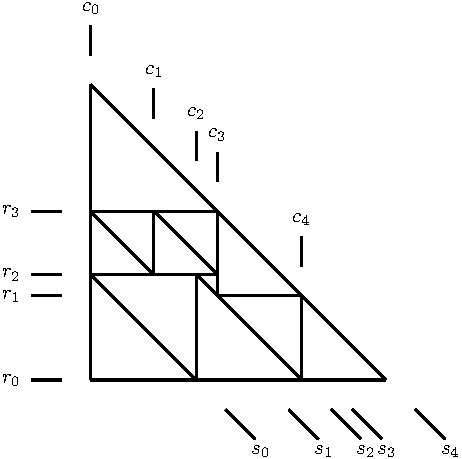
\includegraphics[scale=0.75]{dissection31.pdf}
\end{center}
\caption{Separated dissection for a spherical bitrade. The labels $r_i$, $c_j$,
$s_k$, refer to lines $y = \bar r_i$,
$x = \bar c_j$,
$x+y = \bar s_k$, respectively. The trade $T^{\opa}$ has $12$ entries
and the dissection has $12 + 2 = 14$ vertices.
Applying the transformation $(x,y) \mapsto (y/2 + x, \sqrt 3 y/2)$ gives
an equilateral dissection.}
\label{fg2}
\end{figure} 

\begin{remark}
Suppose that the dissection $\Sigma$ has no vertex of degree $6$.
Pick a vertex $X$ of degree~$4$. If we
move to the right along the row segment to the next vertex $X'$ then we
have $X \tau_1 = X'$. Similarly, moving along the diagonal segments
gives the action of $\tau_2$ and $\tau_3$. If we identify the three vertices of degree $2$
then the dissection encodes, geometrically,
the permutation representation of the bitrade.

If a dissection has a vertex of degree~$6$ then the dissecting triangles
do not (uniquely) define a partial latin square and hence do not encode
a latin bitrade. However, we can recover a separated
bitrade by the following procedure. For each vertex $X$ of degree~$6$,
choose one segment (say, the $r_i$ segment) to stay fixed. Then for the $c_j$
and $s_k$ segments, label the column segment below $X$ with a new name $c'$
and label the symbol segment below $X$ with a new name $s'$. For example,
the centre vertex in Figure~\ref{figsixway} results in the new labels
$c_3$ and $s_3$. The resulting separated bitrade is:
\[ T^{\ast},\, T^{\triangle} =\begin{array}{|c||c|c|c|c|}
\hline \ast & c_0 & c_1 & c_2 & c_3\\
\hline \hline r_0 & s_2 & ~ & s_3 & s_0\\\hline r_1 & s_0 & s_1 & s_2 & s_3\\\hline r_2 & s_1 & s_2 & ~ & ~\\\hline\end{array}\phantom{x}\begin{array}{|c||c|c|c|c|}
\hline \triangle & c_0 & c_1 & c_2 & c_3\\
\hline \hline r_0 & s_0 & ~ & s_2 & s_3\\\hline r_1 & s_1 & s_2 & s_3 & s_0\\\hline r_2 & s_2 & s_1 & ~ & ~\\\hline\end{array}\]
This procedure works for any number of vertices of degree~$6$, as long
as care is taken to only relabel column or symbol segments below a
vertex of degree~$6$ and not to relabel a segment more than
once.\footnote{For a concrete implementation, see 
\texttt{generate\_bitrade\_via\_geometric\_data} in\\
\texttt{triangle\_dissections.py} in \cite{dissections}}
\end{remark}
%%%%%%%%%%%%%%%%%%%%%%%%%%%%%%%%%%%%%%%%%%%%%%%%%%%%%%%%%%%%%%%%%%%%%
\begin{figure}[hbt]
\begin{center}
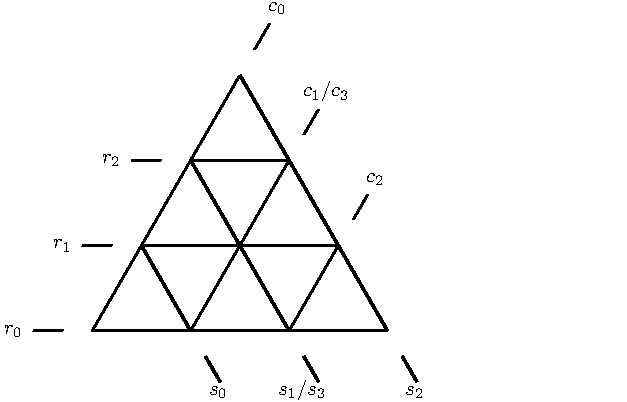
\includegraphics{sixway.pdf}
\end{center}
\caption{A dissection with a vertex of degree $6$.}
\label{figsixway}
\end{figure}
%%%%%%%%%%%%%%%%%%%%%%%%%%%%%%%%%%%%%%%%%%%%%%%%%%%%%%%%%%%%%%%%%%%%% 

Recently Theorem~\ref{sepdissections} has been strengthened to cover
nonseparated as well as separated dissections:

\begin{theorem}[\cite{alesnew}]\label{strongertheorem}
Let $T=(T^\ll, T^\rr)$ be a spherical latin bitrade. Then for 
any $a=(a_1,a_2,a_3) \in T^\ll$, the set $\Delta(T,a)$ of non-degenerate triangles
dissects the triangle
$\Sigma = \{(x,y);$ $x\ge 0$, $y\ge 0$ and $x+y \le 1\}$. The
dissection may not be separated.
\end{theorem}

A fundamental consequence of the theorem is that any dissection of size $s$
can be derived from a pointed spherical bitrade $(T, a)$ of size $s$.
Note that the systems of equations $\eq(T, a)$ have also other
applications: both \cite{nickWanlessBlah} and \cite{alesdissections}
use them to show that every spherical latin trade can be embedded
into a finite abelian group.

\section{Computational results}

Cavenagh and Lison\v ek~\cite{planareulerian} showed that spherical
bitrades are equivalent to planar Eulerian triangulations. To enumerate
triangle dissections we
use plantri~\cite{plantri,plantri2} to enumerate all planar
Eulerian triangulations up to size~$20$ (we also note that
in~\cite{wanlessenumeration} all trades and bitrades have been
enumerated up size~$19$). We wrote a 
plugin~\cite{code} to output the equivalent spherical latin bitrade
$(U^{\opa}, U^{\opb})$ for each triangulation. For each such
$(U^{\opa},U^{\opb})$ we find all
solutions $\eq(T, a)$ for all $a \in T^{\opa}$ and compute each
dissection (in practise this is a list of triangles $\Delta(c,a)$ for
each $c = (c_1,c_2,c_3) \in T^{\rr}$).
To filter out isomorphic dissections we apply all six elements of
the symmetry group for a unit-side equilateral triangle (identity, two rotations,
and three reflections). The {\em canonical signature} of a dissection 
$\Delta(T,a)$ is
the ordered list $[(x,y) \mid (x,y) \textnormal{ is a
vertex of $\Delta(T,a)$}]$. We repeat the whole process for the bitrade $(U^{\opb},U^{\opa})$
because there are spherical latin bitrades where
$(U^{\opa},U^{\opb})$ is not isomorphic to $(U^{\opb},U^{\opa})$. The
final counts for the number of dissections up to isomorphism are found
by simply removing duplicate signatures.

While the solutions to $\eq(T, a)$ exist in the rationals, we find it
easier to work with the final equilateral dissections instead. We use the SymPy package~\cite{sympy} to perform
exact symbolic arithmetic on the canonical form of each dissection.


\subsection{Dissections and automorphism groups}

Using Theorems~\ref{sepdissections} and \ref{strongertheorem}
we have enumerated the number of isomorphism classes of
dissections of size $n \leq 20$. We also record $A(n,k)$, the
number of dissections of size $n$ with
automorphism group of order $k$. See Figures~\ref{figCountSeparated} and
\ref{figCountSeparatedAndNonseparated} for the data. Figure~\ref{logSignatureCounts} has a plot of the 
number of separated dissections with a log scale on the y-axis.

The referee raised the question of asymptotic behaviour. Let us denote
by $d_n$ the number of all dissections of size $n$.  Thus $d_4 = 1$,
$\dots$, $d_{13} = 574$, $\dots$, $d_{20} = 2674753$.  There are some
reasons to believe that $d_n$ can be estimated as $\sigma(n)^n$,
where $\sigma(n)$ is a slowly growing function.  The asymptotic
behaviour of $\sigma(n)$ is not clear yet and is a subject of ongoing
research. Note however that $d_n \ge e_n = (3.43)^{n-8}$ for every
$n\notin \{18,19\}$ such that $8 \le n \le 20$.  If we put $\mu_n =
e_n/d_n$, then in this interval the approximate values of $\mu_n$
are $0.33$, $0.38$, $0.51$, $0.65$, $0.74$, $0.83$, $0.89$, $0.94$,
$0.97$, $0.99$, $1.00$, $1.00$ and $0.99$. The fact that $e_{18}$
and $e_{19}$ are slightly greater than $d_{18}$ and $d_{19}$, while
$e_{20}$ is smaller than $d_{20}$, seems to be surprising.
%
\begin{figure}[htbp]
\begin{center}
\begin{tabular}{|c|c|c|c|c|c|}
\hline $n$ & \# dissections & $A(n,1)$ & $A(n,2)$ & $A(n,3)$ & $A(n,6)$ \\
\hline
\hline 4  & 1 & 0 & 0 & 0 & 1 \\
\hline 6  & 1 & 0 & 1 & 0 & 0 \\
\hline 7  & 2 & 0 & 1 & 0 & 1 \\
\hline 8  & 3 & 2 & 1 & 0 & 0 \\
\hline 9  & 8 & 4 & 4 & 0 & 0 \\
\hline 10 & 20 & 15 & 4 & 0 & 1 \\
\hline 11 & 55 & 47 & 8 & 0 & 0 \\
\hline 12 & 161 & 146 & 15 & 0 & 0 \\
\hline 13 & 478 & 460 & 17 & 0 & 1 \\
\hline 14 & 1496 & 1459 & 37 & 0 & 0 \\
\hline 15 & 4804 & 4746 & 58 & 0 & 0 \\
\hline 16 & 15589 & 15506 & 82 & 0 & 1 \\
\hline 17 & 51377 & 51223 & 154 & 0 & 0 \\
\hline 18 & 172162 & 171923 & 239 & 0 & 0 \\
\hline 19 & 583810 & 583426 & 383 & 0 & 1 \\
\hline 20 & 1998407 & 1997752 & 655 & 0 & 0 \\
\hline 21 & 6902289 & 6901247 & 1042 & 0 & 0 \\
\hline 22 & 24049989 & FIXME & FIXME & FIXME & FIXME \\
\hline 23 & 84364122 & FIXME & FIXME & FIXME & FIXME \\
\hline 24 & 297894288 & FIXME & FIXME & FIXME & FIXME \\
\hline
\end{tabular}
\end{center}
\caption{Number of separated dissections of size $n$, up to isomorphism.
For each $n$, the column $A(n,k)$
records the number of dissections of size $n$ with
automorphism group of order $k$.}
\label{figCountSeparated}
\end{figure}
%
%
\begin{figure}[htbp]
\begin{center}
\begin{tabular}{|c|c|c|c|c|c|}
\hline $n$ & \# dissections & $A(n,1)$ & $A(n,2)$ & $A(n,3)$ & $A(n,6)$ \\
\hline
\hline 4  & 1 & 0 & 0 & 0 & 1 \\
\hline 6  & 1 & 0 & 1 & 0 & 0 \\
\hline 7  & 2 & 0 & 1 & 0 & 1 \\
\hline 8  & 3 & 2 & 1 & 0 & 0 \\
\hline 9  & 9 & 4 & 4 & 0 & 1 \\
\hline 10 & 23 & 15 & 7 & 0 & 1 \\
\hline 11 & 62 & 51 & 11 & 0 & 0 \\
\hline 12 & 188 & 162 & 25 & 0 & 1 \\
\hline 13 & 574 & 532 & 39 & 0 & 3 \\
\hline 14 & 1826 & 1745 & 81 & 0 & 0 \\
\hline 15 & 5953 & 5795 & 157 & 0 & 1 \\
\hline 16 & 19664 & 19380 & 277 & 2 & 5 \\
\hline 17 & 66049 & 65489 & 560 & 0 & 0 \\
\hline 18 & 224700 & 223625 & 1070 & 0 & 5 \\
\hline 19 & 771859 & 769851 & 1992 & 8 & 8 \\
\hline 20 & 2674753 & 2670755 & 3998 & 0 & 0 \\
\hline
\end{tabular}
\end{center}
\caption{Lower bounds on the number of separated and nonseparated dissections of size $n$, up to isomorphism.
For each $n$, the column $A(n,k)$
records the number of dissections of size $n$ with
automorphism group of order $k$.}
\label{figCountSeparatedAndNonseparated}
\end{figure}
%

\begin{figure}[htbp]
\begin{center}
\resizebox{12cm}{!}{\includegraphics{signature_counts.pdf}}
\end{center}
\caption{Number of separated dissections up to size $24$.}
\label{logSignatureCounts}
\end{figure}



\subsection{Perfect dissections}

%Equilateral triangles can tile in an up or down direction, depending on
%whether the vertex opposite the triangle's horizontal side is above or
%below the horizontal side. If these triangles are considered to be
%different since they are not congruent (even though they are of the same
%size) then we get the notion of a {\em perfect tiling} or {\em perfect
%dissection}~\cite{squaring}.

Using our enumeration code we can confirm W.~T. Tutte's
conjecture~\cite{MR0003040,MR0027521}
that the smallest perfect dissection has size $15$ (see
Figure~\ref{figPerfect15}).
The perfect dissections of size $16$ and $17$ are shown in
Figures~\ref{figPerfect16} and \ref{figPerfect17}.
%
\begin{figure}[htbp]
\begin{center}
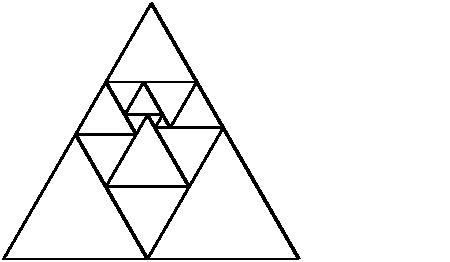
\includegraphics{output-dissections-perfect-dissection15_i442079_r7_c4.pdf}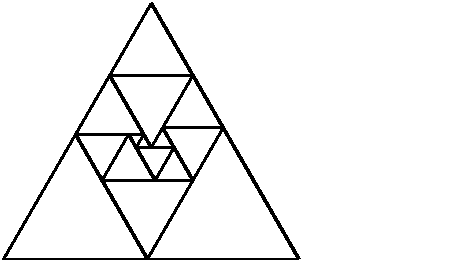
\includegraphics{output-dissections-perfect-dissection15_i442079_r7_c6.pdf}
\end{center}
\caption{The two perfect dissections of size $15$.}
\label{figPerfect15}
\end{figure}
%
\begin{figure}[htbp]
\begin{center}
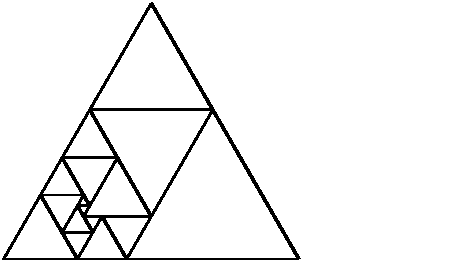
\includegraphics{output-dissections-perfect-dissection16_i128609_r5_c0.pdf}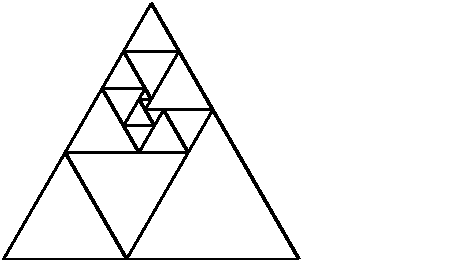
\includegraphics{output-dissections-perfect-dissection16_i129387_r1_c3.pdf} 
\end{center}
\caption{The two perfect dissections of size $16$.}
\label{figPerfect16}
\end{figure}
%
\begin{figure}[htbp]
\begin{center}
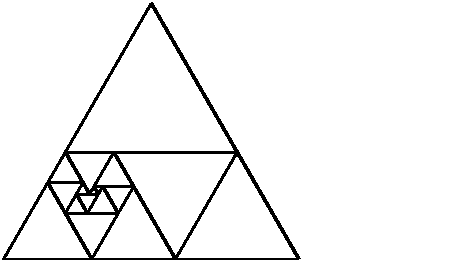
\includegraphics{output-dissections-perfect-dissection17_i442068_r3_c4.pdf}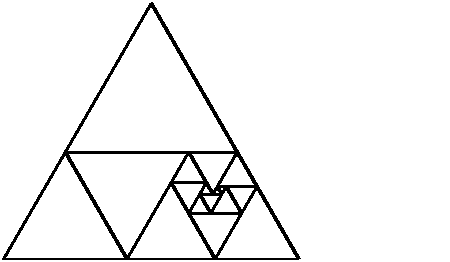
\includegraphics{output-dissections-perfect-dissection17_i442068_r3_c5.pdf}
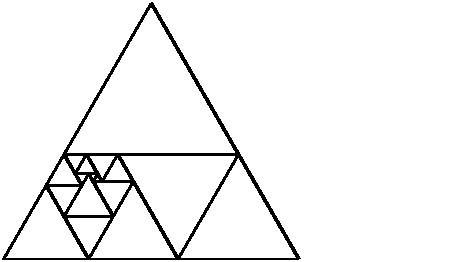
\includegraphics{output-dissections-perfect-dissection17_i442083_r6_c4.pdf}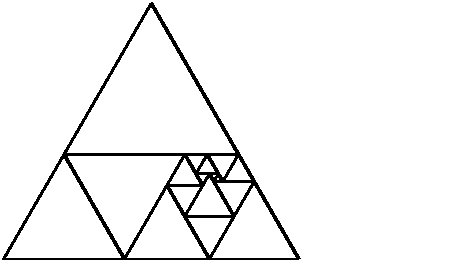
\includegraphics{output-dissections-perfect-dissection17_i442083_r6_c7.pdf}
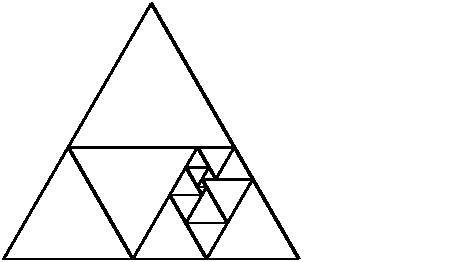
\includegraphics{output-dissections-perfect-dissection17_i455488_r2_c5.pdf}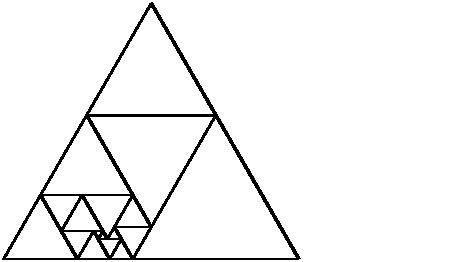
\includegraphics{output-dissections-perfect-dissection17_i483193_r2_c6.pdf}
\end{center}
\caption{The six perfect dissections of size $17$.}
\label{figPerfect17}
\end{figure}
%
The perfect dissections of size up to $20$ are available in PDF format~\cite{dissections}.
The following table summarises the known number of isomorphism classes
of perfect dissections:

\begin{center}
\begin{tabular}{|c|c|}
\hline $n$ & \# perfect dissections \\
\hline
\hline 15 & 2 \\
\hline 16 & 2 \\
\hline 17 & 6 \\
\hline 18 & 23 \\
\hline 19 & 64 \\
\hline 20 & 181 \\
\hline
\end{tabular}
\end{center}

It is an open problem to determine if there exists a nonseparated
perfect dissection. If such a dissection exists then it will have size
greater than $20$.

\subsection{Other observations}

There exist bitrades of size $n \geq 10$ for which there is no
separated dissection of size $n$. The following table shows a sample
of these bitrades, giving the sizes of all possible dissections for
the particular bitrade of size $n$.

\begin{center}
\begin{tabular}{|c|l|}
\hline
$n$ & size of possible dissections \\
\hline
\hline 10 & 4, 7  \\
\hline 12 & 4, 7, 8, 9  \\
\hline 12 & 4, 9, 11  \\
\hline 12 & 4, 11  \\
\hline 12 & 6, 9  \\
\hline 12 & 9  \\
\hline 12 & 11  \\
\hline 13 & 4, 7  \\
\hline 13 & 4, 7, 9, 10  \\
\hline 13 & 4, 7, 10  \\
\hline 13 & 4, 9, 10, 12  \\
\hline 13 & 4, 11, 12  \\
\hline 13 & 9, 10, 12  \\
\hline 13 & 10, 11  \\
\hline
\end{tabular}
\end{center}

A {\em trivial dissection} has triangles of only one size. Apart from
$n = 4$, all trivial dissections are nonseparated.  The following
table lists lower bounds on the number of bitrades that give rise to
the (unique) separated dissection of size $n$ (naturally we allow for
nonseparated solutions to find these trivial dissections).

\begin{center}
\begin{tabular}{|c|l|}
\hline
$n$ & lower bound on number of source bitrades \\
\hline
\hline 4 & 2380591 \\
\hline 8 & 111890 \\
\hline 13 & 1321 \\ 
\hline
\end{tabular}
\end{center}

For each size $n$ we collect examples of dissections with the largest
relative difference in size between the largest and smallest triangle in
the dissection. In all cases the smallest triangle has size $1$ and the
largest triangle  is given in the second column of the table below:

\begin{center}
\begin{tabular}{|c|c|c|c|}
\hline
$n$ & size of largest triangle \\
\hline
\hline 4 & 1 \\
\hline 6 & 2 \\
\hline 7 & 2 \\
\hline 8 & 3 \\
\hline 9 & 4 \\
\hline 10 & 5 \\
\hline 11 & 7 \\
\hline 12 & 9 \\
\hline 13 & 12 \\
\hline 14 & 16 \\
\hline 15 & 21 \\
\hline 16 & 28 \\
\hline 17 & 37 \\
\hline 18 & 49 \\
\hline 19 & 67 \\
\hline 20 & 91 \\
\hline
\end{tabular}
\end{center}

The dissections that give rise to these maximum ratios are shown below
(sorted by dissection size $n$):

\begin{center}
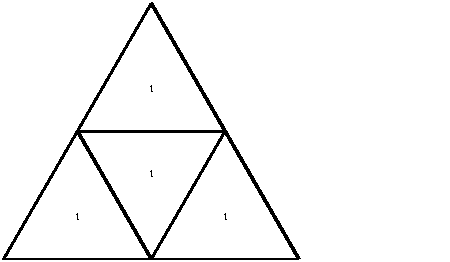
\includegraphics{max_relative_size_4.pdf}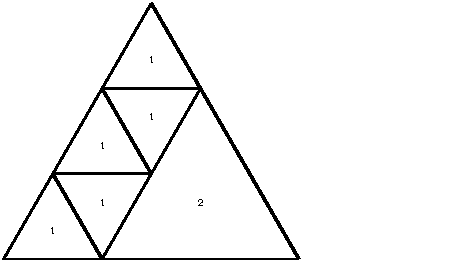
\includegraphics{max_relative_size_6.pdf}
\end{center}
\begin{center}
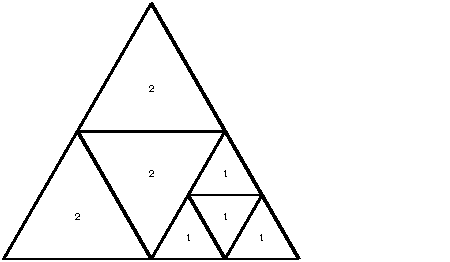
\includegraphics{max_relative_size_7.pdf}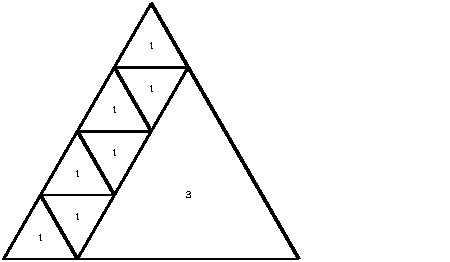
\includegraphics{max_relative_size_8.pdf}
\end{center}
\begin{center}
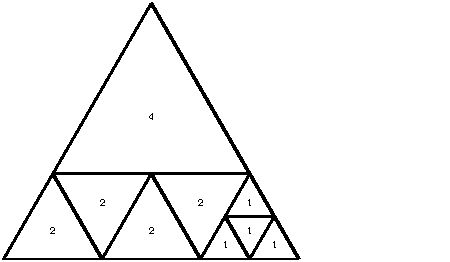
\includegraphics{max_relative_size_9.pdf}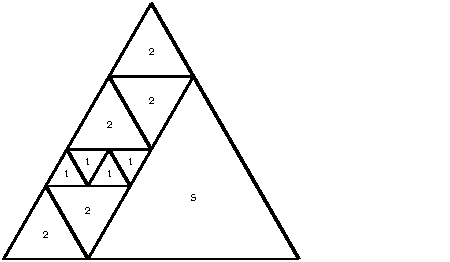
\includegraphics{max_relative_size_10.pdf}
\end{center}
\begin{center}
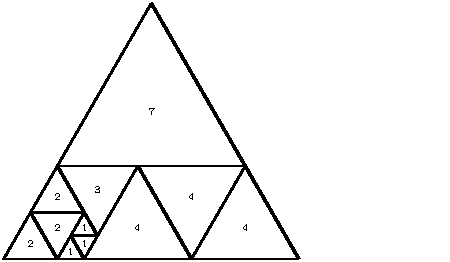
\includegraphics{max_relative_size_11.pdf}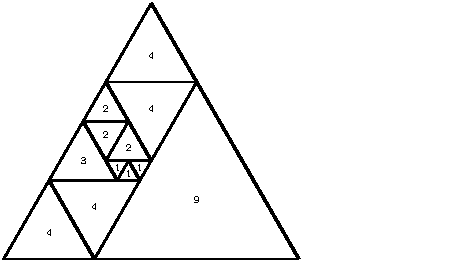
\includegraphics{max_relative_size_12.pdf}
\end{center}
\begin{center}
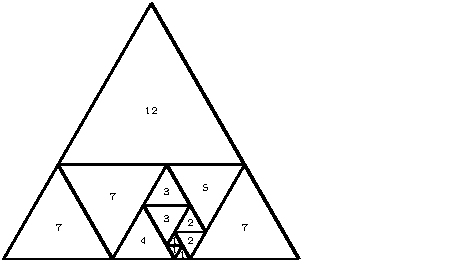
\includegraphics{max_relative_size_13.pdf}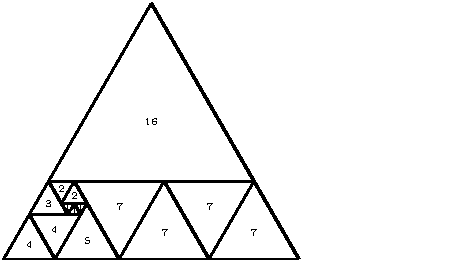
\includegraphics{max_relative_size_14.pdf}
\end{center}
\begin{center}
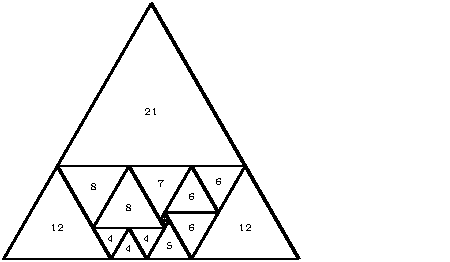
\includegraphics{max_relative_size_15.pdf}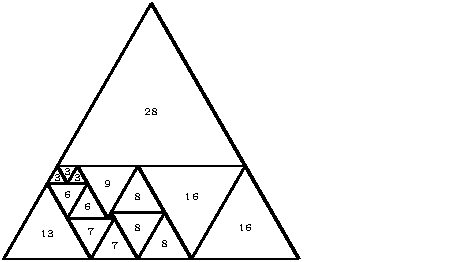
\includegraphics{max_relative_size_16.pdf}
\end{center}
\begin{center}
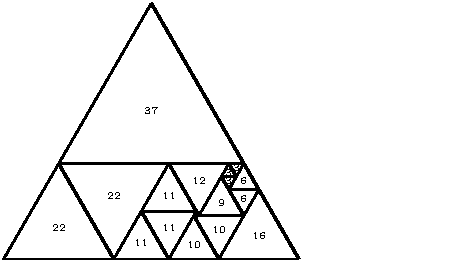
\includegraphics{max_relative_size_17.pdf}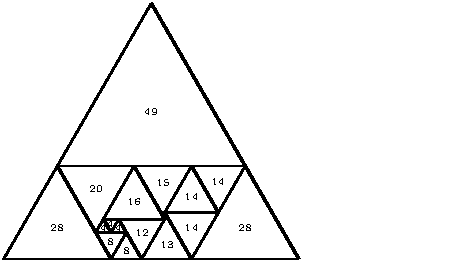
\includegraphics{max_relative_size_18.pdf}
\end{center}
\begin{center}
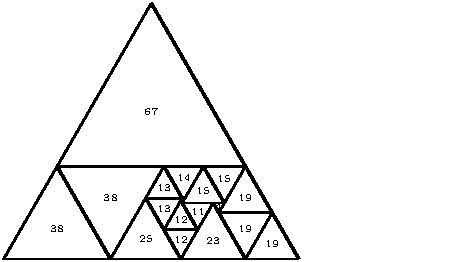
\includegraphics{max_relative_size_19.pdf}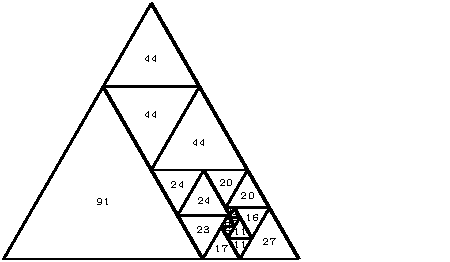
\includegraphics{max_relative_size_20.pdf}
\end{center}

\clearpage

%\bibliographystyle{elsarticle-num}
%\bibliography{dissection_enumeration}

\begin{thebibliography}{10}
\expandafter\ifx\csname url\endcsname\relax
  \def\url#1{\texttt{#1}}\fi
\expandafter\ifx\csname urlprefix\endcsname\relax\def\urlprefix{URL }\fi
\expandafter\ifx\csname href\endcsname\relax
  \def\href#1#2{#2} \def\path#1{#1}\fi

\bibitem{plantri}
G.~Brinkmann, B.~D. McKay, plantri (software),
  \url{http://cs.anu.edu.au/∼bdm/plantri}.

\bibitem{plantri2}
G.~Brinkmann, B.~D. McKay, Fast generation of some classes of planar
graphs, Electronic Notes in Discrete Mathematics 3 (1999) 28--31.
  \url{http://cs.anu.edu.au/∼bdm/plantri}.

\bibitem{MR0003040}
R.~L. Brooks, C.~A.~B. Smith, A.~H. Stone, W.~T. Tutte, The dissection of
  rectangles into squares, Duke Math. J. 7 (1940) 312--340.

\bibitem{planareulerian}
N.~J. Cavenagh, P.~Lison\v ek, Planar eulerian triangulations are equivalent to
  spherical latin bitrades, J. Comb. Theory, Ser. A 115~(1) (2008) 193--197.

\bibitem{nickWanlessBlah}
N.~J. Cavenagh, I.~M. Wanless, Latin trades in groups defined on planar
  triangulations, J. Algebraic Combin. 30 (2009) 323--347.

\bibitem{wanlesshandbook}
C.~J. Colbourn, J.~H. Dinitz, I.~M. Wanless, Handbook of combinatorial designs,
  Chapman \& Hall/CRC, Boca Raton, FL, 2007.

\bibitem{alesnew}
A.~Dr{\'a}pal, Dissections of equilateral triangles and pointed spherical latin
  bitrades, submitted.

\bibitem{ales-geometrical}
A.~Dr{\'a}pal, Geometrical structure and construction of latin trades, Advances
  in Geometry 9~(3) (2009) 311--348.

\bibitem{Dr9}
A.~Dr{\'a}pal, Geometry of latin trades, manuscript circulated at the
  conference Loops, Prague (2003).

\bibitem{aleshamming}
A.~Dr{\'a}pal, Hamming distances of groups and quasi-groups, Discrete Math.
  235~(1-3) (2001) 189--197, combinatorics (Prague, 1998).

\bibitem{alesdissections}
A.~Dr{\'a}pal, V.~Kala, C.~H\"{a}m\"{a}l\"{a}inen, Latin bitrades,
  dissections of equilateral triangles and abelian groups,
  Journal of Combinatorial Designs, Volume 18 Issue 1 (2010), 1--24.

\bibitem{hamalainen2007}
C.~H\"{a}m\"{a}l\"{a}inen, Latin bitrades and related structures, {PhD} in
  {M}athematics, Department of Mathematics, The University of Queensland,
  http://carlo-hamalainen.net/phd/hamalainen-20071025.pdf (2007).

\bibitem{code}
C.~H\"{a}m\"{a}l\"{a}inen, Spherical bitrade enumeration code,
  \url{http://bitbucket.org/carlohamalainen/spherical}.

\bibitem{dissections}
C.~H\"{a}m\"{a}l\"{a}inen,
Triangle dissections code,
  \url{http://bitbucket.org/carlohamalainen/dissections}.

\bibitem{MR1092545}
M.~Laczkovich, Tilings of polygons with similar triangles, Combinatorica 10~(3)
  (1990) 281--306.

\bibitem{MR1794696}
J.~D. Skinner, C.~A.~B. Smith, W.~T. Tutte, On the dissection of rectangles
  into right-angled isosceles triangles, J. Combin. Theory Ser. B 80~(2) (2000)
  277--319.

\bibitem{sympy}
{SymPy Development Team}, \href{http://www.sympy.org}{SymPy: Python library for
  symbolic mathematics} (2009).
\newline\urlprefix\url{http://www.sympy.org}

\bibitem{squaring}
Tiling by similar triangles, \url{http://www.squaring.net/tri/twt.html}.

\bibitem{MR0027521}
W.~T. Tutte, The dissection of equilateral triangles into equilateral
  triangles, Proc. Cambridge Philos. Soc. 44 (1948) 463--482.

\bibitem{wanlessenumeration}
Ian~M. Wanless.
\newblock A computer enumeration of small {L}atin trades.
\newblock {\em Australas. J. Combin.}, 39:247--258, 2007.


\end{thebibliography}

\clearpage

\section*{Appendix A: Triangle dissections}

Here we present representatives of the isomorphism classes of triangle
dissections of size $n \in \{4, 6, 7, 8, 9, 10 \}$.

%Unused now
%\input{data_unique_dissections.tex}

\subsection*{$n = 4$}

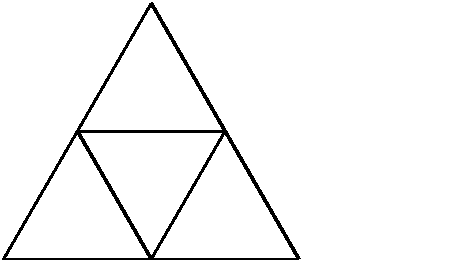
\includegraphics{output-dissections-dissection4_i36_r3_c1.pdf}

\subsection*{$n = 6$}

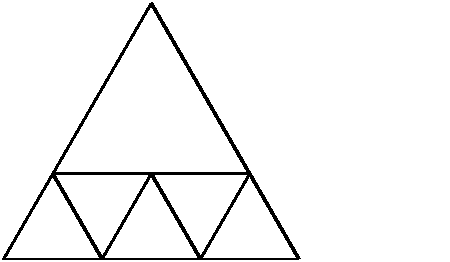
\includegraphics{output-dissections-dissection6_i41_r1_c3.pdf}

\subsection*{$n = 7$}

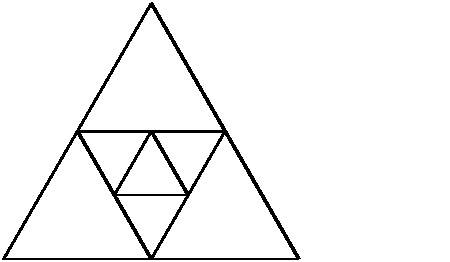
\includegraphics{output-dissections-dissection7_i27_r3_c2.pdf}
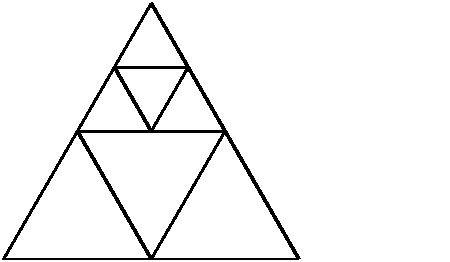
\includegraphics{output-dissections-dissection7_i29_r1_c2.pdf}

\subsection*{$n = 8$}

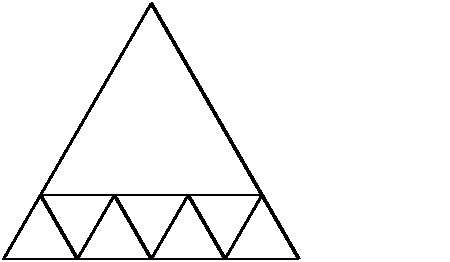
\includegraphics{output-dissections-dissection8_i31_r2_c4.pdf}
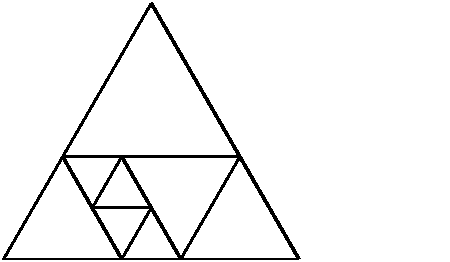
\includegraphics{output-dissections-dissection8_i37_r2_c2.pdf}
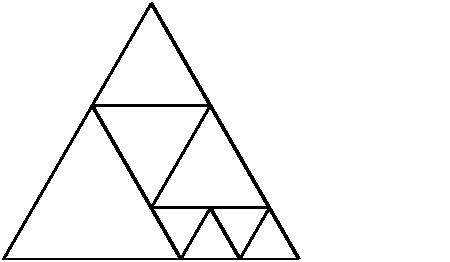
\includegraphics{output-dissections-dissection8_i37_r2_c4.pdf}

\subsection*{$n = 9$}

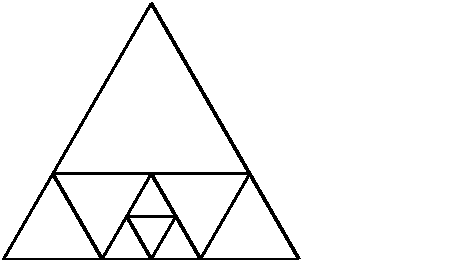
\includegraphics{output-dissections-dissection9_i10_r0_c2.pdf}
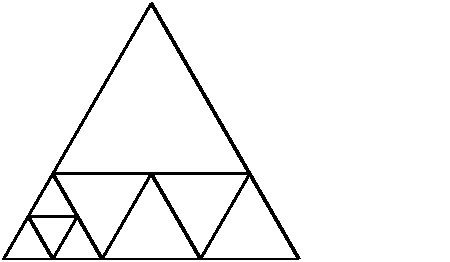
\includegraphics{output-dissections-dissection9_i10_r0_c3.pdf}
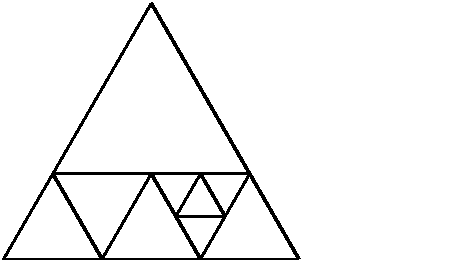
\includegraphics{output-dissections-dissection9_i10_r2_c2.pdf}
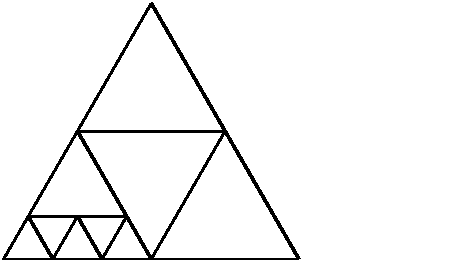
\includegraphics{output-dissections-dissection9_i11_r0_c3.pdf}
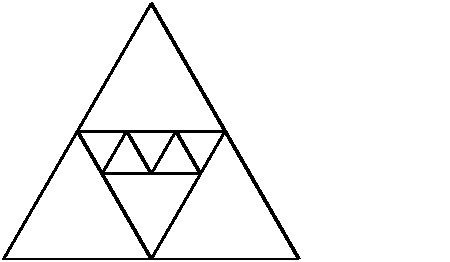
\includegraphics{output-dissections-dissection9_i11_r1_c0.pdf}
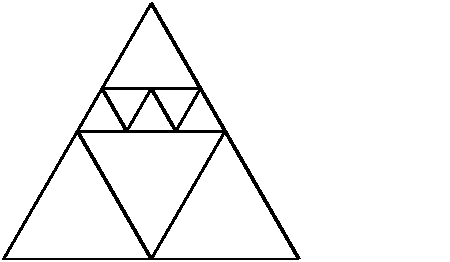
\includegraphics{output-dissections-dissection9_i11_r1_c3.pdf}
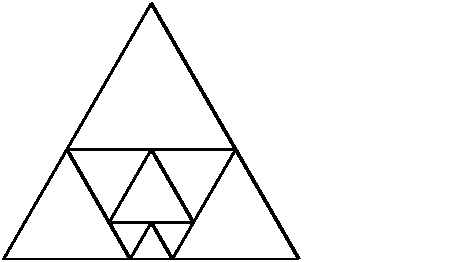
\includegraphics{output-dissections-dissection9_i13_r2_c1.pdf}
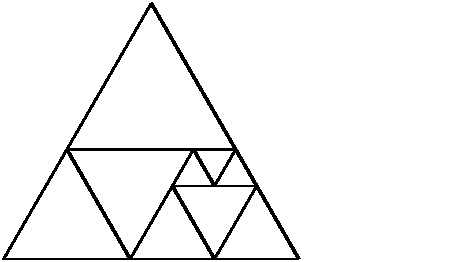
\includegraphics{output-dissections-dissection9_i13_r2_c3.pdf}
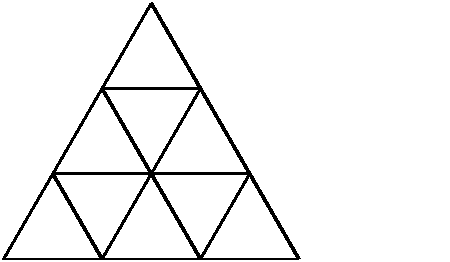
\includegraphics{output-dissections-dissection9_i45_r0_c0.pdf}

\subsection*{$n = 10$}

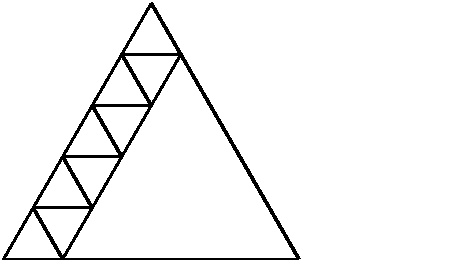
\includegraphics{output-dissections-dissection10_i15_r4_c1.pdf}
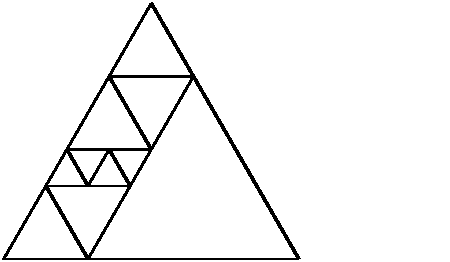
\includegraphics{output-dissections-dissection10_i17_r1_c0.pdf}
\includegraphics{output-dissections-dissection10_i17_r1_c1.pdf}
\includegraphics{output-dissections-dissection10_i17_r3_c0.pdf}
\includegraphics{output-dissections-dissection10_i17_r3_c1.pdf}
\includegraphics{output-dissections-dissection10_i17_r3_c2.pdf}
\includegraphics{output-dissections-dissection10_i19_r2_c3.pdf}
\includegraphics{output-dissections-dissection10_i19_r3_c1.pdf}
\includegraphics{output-dissections-dissection10_i19_r3_c3.pdf}
\includegraphics{output-dissections-dissection10_i21_r1_c2.pdf}
\includegraphics{output-dissections-dissection10_i21_r1_c3.pdf}
\includegraphics{output-dissections-dissection10_i21_r2_c2.pdf}
\includegraphics{output-dissections-dissection10_i21_r2_c3.pdf}
\includegraphics{output-dissections-dissection10_i23_r3_c0.pdf}
\includegraphics{output-dissections-dissection10_i23_r3_c1.pdf}
\includegraphics{output-dissections-dissection10_i23_r3_c2.pdf}
\includegraphics{output-dissections-dissection10_i25_r0_c0.pdf}
\includegraphics{output-dissections-dissection10_i25_r1_c0.pdf}
\includegraphics{output-dissections-dissection10_i25_r1_c3.pdf}
\includegraphics{output-dissections-dissection10_i26_r0_c3.pdf}
\includegraphics{output-dissections-dissection10_i29_r2_c0.pdf}
\includegraphics{output-dissections-dissection10_i29_r2_c3.pdf}
\includegraphics{output-dissections-dissection10_i45_r3_c1.pdf}

\clearpage

\section*{Appendix B: Further Analysis}

The questions in this appendix were suggested by 
Stuart Anderson\footnote{\texttt{stuart.errol.anderson@gmail.com} and
\url{http://www.squaring.net/}} (personal communication with Carlo Hamalainen).

\begin{itemize}

\item What is the range of sides for dissected triangles across and
between orders? 

See pp\_triangle\_sizes.cpp

\item What is the range of sizes for elements of dissected triangles
across and between orders?

See pp\_dissection\_element\_sizes.cpp

\item Do isomers (same elements arranged differently) exist? What is
the minimum order?

See pp\_isomer\_sigs; there seem to exist isomers for each order geq
7, can use pp\_isomer\_sigs to count the number of isomer classes
for each order. Another sequence...

\item Do disjoint-ntuples exist (same size triangles, same number of
elements, all different sizes) can we make the equivalent of compound
perfect squares with compound perfect triangled triangles composed
of disjoint n-tuples?

\item What is the smallest order compound triangled triangle that can
be made? (I guess it would be 29, Tuttes order 15 enlarged and put
inside itself, unless there's another way to do it with fewer squares,
i havnt really thought about it)

\item What is the smallest triangle that can exist on a corner, or
on the boundary? (for squared squares its 5 on the boundary and 9
on a corner and those squares are extremely rare, order 44, Gambini
found them)

\item Can the largest element be completely in the interior? (this
is possible for squared squares) If possible, smallest order?

Yes, two examples of order 18, see pp\_largest\_in\_interior.cpp

\item How high can you get in ratio between the smallest element and
the largest? (try to make or find a tiling where the smallest element
is as large as possible (compared to the largest)

See ./pp\_ratio\_spectrum.cpp for a count of all ratios of largest/smallest.

See also pp\_plot\_ratio\_spectrum.py for plotting the output of ./pp\_ratio\_spectrum.cpp 

\item What is the distribution of odd and even elements by order?
is the distribution mod 3 more relevant?

\item What is the distribution of prime numbers as triangle elements?
(squared square elements appear to have a normal distribution) Lots
of questions....

\end{itemize}

\clearpage
\subsection*{B.1 blah}

\begin{center}
\resizebox{12cm}{!}{\includegraphics{signature_counts.pdf}}
\end{center}

\begin{center}
\resizebox{12cm}{!}{\includegraphics{pp_ratio_spectrum_4.pdf}}
\end{center}

\begin{center}
\resizebox{12cm}{!}{\includegraphics{pp_ratio_spectrum_6.pdf}}
\end{center}

\begin{center}
\resizebox{12cm}{!}{\includegraphics{pp_ratio_spectrum_7.pdf}}
\end{center}

\begin{center}
\resizebox{12cm}{!}{\includegraphics{pp_ratio_spectrum_8.pdf}}
\end{center}

\begin{center}
\resizebox{12cm}{!}{\includegraphics{pp_ratio_spectrum_9.pdf}}
\end{center}

\begin{center}
\resizebox{12cm}{!}{\includegraphics{pp_ratio_spectrum_10.pdf}}
\end{center}

\begin{center}
\resizebox{12cm}{!}{\includegraphics{pp_ratio_spectrum_11.pdf}}
\end{center}

\begin{center}
\resizebox{12cm}{!}{\includegraphics{pp_ratio_spectrum_12.pdf}}
\end{center}

\begin{center}
\resizebox{12cm}{!}{\includegraphics{pp_ratio_spectrum_13.pdf}}
\end{center}

\begin{center}
\resizebox{12cm}{!}{\includegraphics{pp_ratio_spectrum_14.pdf}}
\end{center}

\begin{center}
\resizebox{12cm}{!}{\includegraphics{pp_ratio_spectrum_15.pdf}}
\end{center}

\begin{center}
\resizebox{12cm}{!}{\includegraphics{pp_ratio_spectrum_16.pdf}}
\end{center}

\begin{center}
\resizebox{12cm}{!}{\includegraphics{pp_ratio_spectrum_17.pdf}}
\end{center}

\begin{center}
\resizebox{12cm}{!}{\includegraphics{pp_ratio_spectrum_18.pdf}}
\end{center}

\begin{center}
\resizebox{12cm}{!}{\includegraphics{pp_ratio_spectrum_19.pdf}}
\end{center}

\begin{center}
\resizebox{12cm}{!}{\includegraphics{pp_ratio_spectrum_20.pdf}}
\end{center}

\begin{center}
\resizebox{12cm}{!}{\includegraphics{pp_ratio_spectrum_21.pdf}}
\end{center}

\begin{center}
\resizebox{12cm}{!}{\includegraphics{pp_ratio_spectrum_22.pdf}}
\end{center}

\begin{center}
\resizebox{12cm}{!}{\includegraphics{pp_ratio_spectrum_23.pdf}}
\end{center}

\begin{center}
\resizebox{12cm}{!}{\includegraphics{pp_ratio_spectrum_24.pdf}}
\end{center}


\subsection*{B.2 bleh}

\end{document}









